\chapter{Introdução}

Na atualidade a segurança e bem estar das pessoas é um aspecto fundamental a ser garantido, ainda mais para trabalhadores em ambientes industriais, onde os riscos são mais severos. Diversas normas e regras existem no sentido de garantir que essa condição seja atendida. Com a progressão dos meios tecnológicos novas ferramentas surgiram para facilitar as medidas de controle e proteger as pessoas.

Um caso concreto para aplicação dessas ferramentas ocorre na Wanke, indústria de eletrodomésticos de Indaial-SC, que conta com pontes rolantes, um sistema de transporte que facilita a movimentação de peças no meio industrial. Esse instrumento permite carregar moldes de até centenas de kilogramas entre estações de trabalho. É um fator de preocupação que um desses moldes se solte ou contenha peças livres que caiam e firam algum funcionário. 

Esse trabalho pretende elaborar um sistema automático de detecção de pessoas que possibilite impedir que a ponte rolante se movimente enquanto houver colaboradores sob sua área de movimentação. Essa detecção é feita com base em imagens de profundidade e algoritmos de aprendizado de máquina. As imagens são obtidas através de uma câmera stereo de maneira que o valor de cada pixel representa a distância entre a câmera e o objeto. 

Os aspectos fundamentais e um comparativo entre técnicas tradicionais e de aprendizado profundo é apresentado. O resultado das diferentes técnicas em figuras de mérito específicas para classificação é destacado.

\section{Aprendizado de máquina}
Segundo Arthur Samuel, aprendizado de máquina é o ramo da inteligência artificial que estuda técnicas que possibilitam um computador realizar uma tarefa sem ser explicitamente programado para desempenhá-la. 

Mitchell (1997) define: "Se diz que um computador aprende com uma experiência $E$ com respeito a uma tarefa $T$ e medida de performance $P$ a medida que a performance medida por $P$ medida em uma tarefa $T$ progride com a experiência $E$". 

Entre as tarefas pode-se citar classificação, em que uma amostra deve ser atribuída a uma das classes apresentadas; regressão, em que uma amostra deve ser mapeada em um valor real; síntese, onde o algoritmo deve gerar novas amostras que sejam similares às de entrada.

As medidas de performance são específicas da tarefa em questão e seu uso deve variar com a aplicação. Para conjuntos de dados simples e balanceados uma medida comum a classificadores é a Exatidão Geral (EG), razão do número correto de classificações pelo número total. Porém a Exatidão Específica (EE), razão das classificações corretas pelo número total da classe, fornece maiores indicativos sobre o potencial discriminativo do algoritmo. Para problemas de regressão podem ser adotadas as medidas de erro médio quadrático.

As experiências são o conjunto de dados que o algoritmo utiliza para aprender, aqui também chamado de \textit{dataset}. Esse conjunto de dados é dito supervisionado quando possui um indicador da classe que cada amostra pertence ou o valor esperado para aquela amostra, no caso de regressão. Para um conjunto não supervisionado, espera-se aprender mais sobre a distribuição dos dados. Isso permite, por exemplo, detectar amostras anômalas e dividir o conjunto de dados em grupos (\textit{clusters}) que apresentem alguma similaridade estrutural.

Uma experiência, também chamada de exemplo ou amostra, é uma coleção de descrições, obtida através de um descritor de características, figura \ref{fig:features}. Essa descrição é obtida através de um processo que pode mensurar alguma grandeza específica de algum objeto ou evento. Para o campo de imagens são comuns descritores de borda e histograma de cores. Em geral, um descritor busca obter uma representação compacta, reduzindo dimensionalidade, e discrimantiva entre as amostras de maneira a facilitar a etapa de classificação. A etapa de extração de características pode ser vista como um préprocessamento ou transformação para um domínio de maior relevância.

\begin{figure}[h]
\caption{Exemplo de descritores: histograma de bordas e cores}
\centering
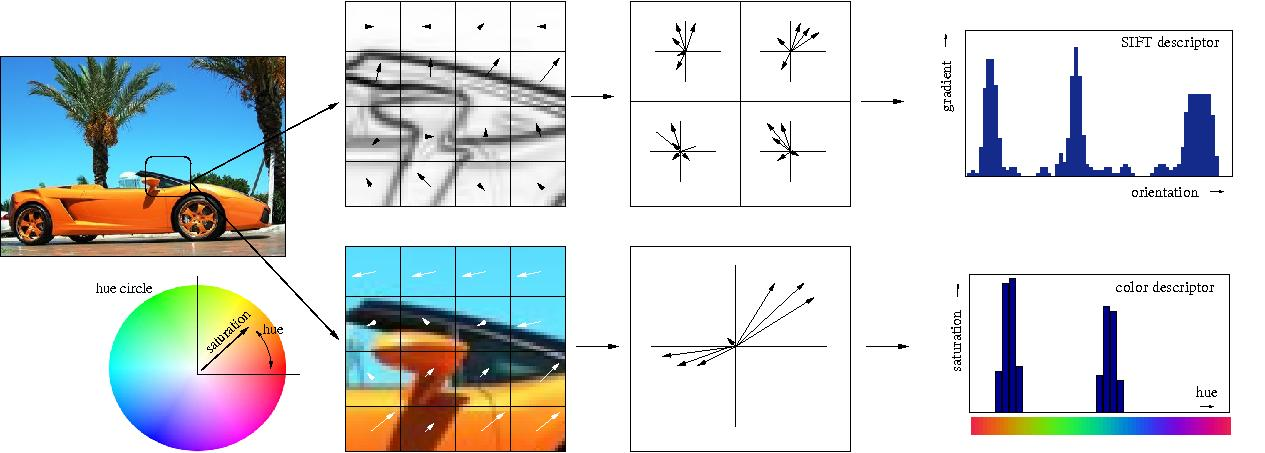
\includegraphics[width=0.8\textwidth]{features}
\label{fig:features}
\end{figure}

\section{Métodos clássicos}
O problema de classificação de objetos é um clássico no campo de visão computacional e requer aprendizado de máquina. Uma abordagem tradicional consiste nos seguintes passos.
	\begin{enumerate}
	\item Identificar uma região de interesse no caso de uma imagem com múltiplos objetos.
	\item Utilizar um extrator de características para descrição do objeto.
	\item Introduzir a amostra, proveniente do descritor, em um classificador simples, obtendo a classe correspondente.
	\end{enumerate}

Métodos tradicionais são superficiais a medida que requerem que um extrator de características seja utilizado antes da classificação. Isso se deve à necessidade de reduzir a dimensionalidade das amostras e discriminar classes diferentes, o que possibilita ganhos de performance com baixa complexidade do classificador.

A escolha do descritor está diretamente ligada com a qualidade do processo de classificação. Um descritor é criado especificamente para uma aplicação e dificilmente pode ser utilizado em outros campos: um descritor para imagens não consegue entender um sinal de áudio. Assim, sua concepção demanda conhecimento e prática de especialistas da área de aplicação. Para um problema de classificação entre imagens de bananas e maçãs, por exemplo, um descritor relacionado a cor teria maior relevância do que a de bordas.

% SVM
Após ter uma representação adequada das experiências escolhe-se o tipo do classificador. O modelo de \textit{Support Vector Machines} é bastante utilizado pois possui representação e uso simplificado e demonstrou bons resultados ao tratar amostras de dimensões medianas (ordem de centenas) com um dataset pequeno (ordem de milhares de amostras) sem ajuste fino. Seu modelo consiste em encontrar um hiperplano de separação entre classes ótimo, no sentido de maximizar a distância entre as amostras e o hiperplano. As amostras mais próximas do hiperplano são chamadas vetores suportes, como mostrado na figura \ref{fig:svm-hyperplane}.

\begin{figure}[h]
\caption{Hiperplano ótimo para separação das classes}
\centering
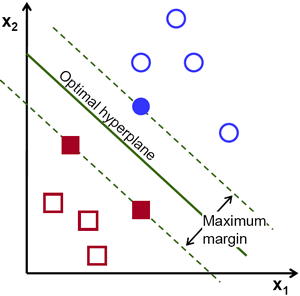
\includegraphics[width=0.5\textwidth]{svm/svm-hyperplane}
\label{fig:svm-hyperplane}
\end{figure}

Para amostras com distribuição complexa a possibilidade de não existir um hiperplano que consiga separar o conjunto satisfatóriamente é grande. Para resolver esse problema emprega-se uma função que mapeia essas amostras para um espaço de maior dimensionalidade em que as classes sejam linearmente separáveis.

\section{Aprendizado profundo}
As redes neurais artificiais foram inspiradas no entendimento rudimentar dos neurônios biológicos ainda na década de 1950, porém não mais pretende obter um modelo fiel do sistema biológico mas em obter bons resultados para tarefas de aprendizado de máquina. Suas estruturas eram então compostas por um único elemento chamado \textit{perceptron}, um modelo matemático que recebe múltiplas entradas, faz um somatório ponderado por parâmetros associados a cada entrada e então aplica uma função não-linear, chamada função de ativação, para retornar uma única saída.

\begin{figure}[h]
\caption{A estrutura de um perceptron}
\centering
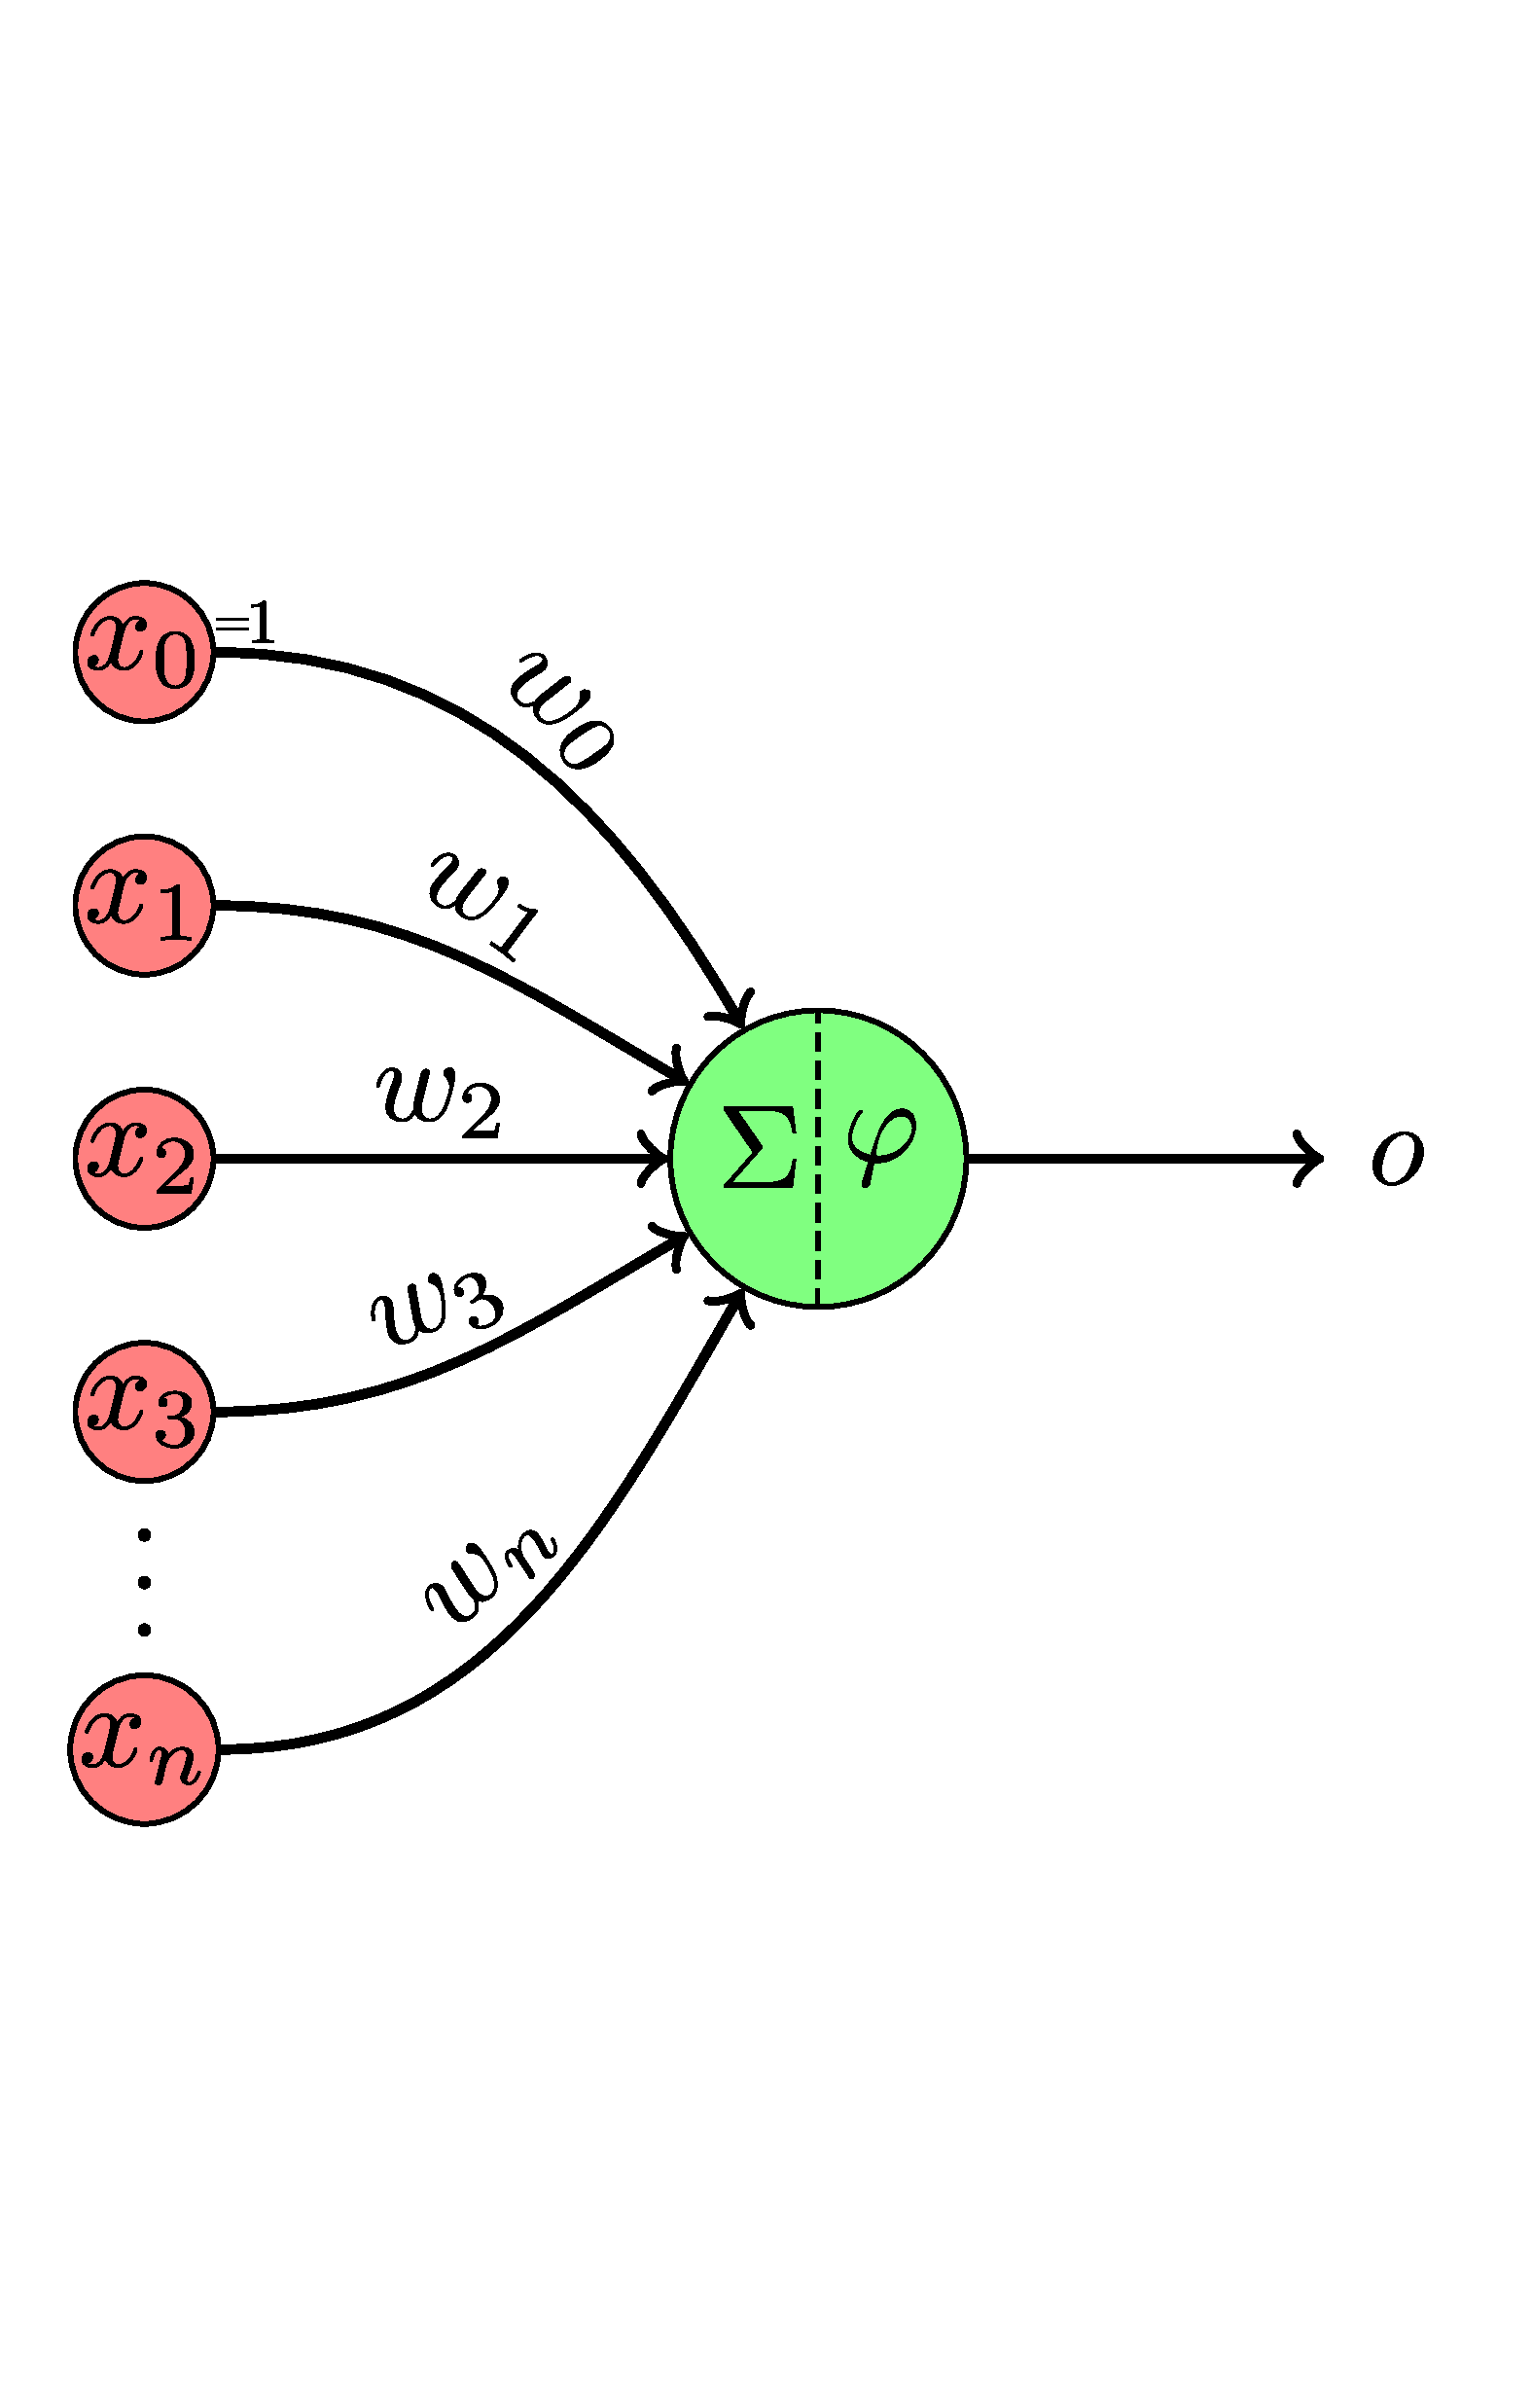
\includegraphics[width=0.4\textwidth]{perceptron}
\label{fig:perceptron}
\end{figure}

Alguns problemas impediram os avanços desse classificador, a destacar: a incapacidade de aprender uma tarefa comum como o ou-exclusivo (dado que os dados não são linearmente separáveis) e o baixo poder de processamento dos computadores da época.

A partir da década de 1970 com o aumento drástico da capacidade computacional essa estrutura ganhou complexidade e passou a ser integrada por múltiplos \textit{perceptrons} organizados em camadas, o que possibilitou aprender datasets mais desafiadores. Foi esse evento que iniciou a jornada para o advento das técnicas de aprendizado profundo.

Em contraposição com métodos tradicionais, em que é necessário criar um extrator de características manualmente, métodos profundos permitem que a amostra seja alimentada ao classificador sem préprocessamento. Isso é possível pois internamente o sistema gera um descritor ótimo para discriminação das amostras. Ou seja, o próprio classificador encontra a melhor maneira de representar as amostras para obter um bom resultado, economizando tempo e acabando com a necessidade de especialistas em criar esses descritores. %Referencia apresentação LeCun

Outros autores também afirmam que o método é chamado profundo pois pressupõe um grande número de camadas intermediárias. O preço a pagar por não precisar criar um descritor manual específico para uma aplicação é a maior complexidade do sistema e o grande volume de amostras necessárias para o treinamento do classificador.

\subsection{Perceptron multicamadas (MLP)}
A evolução do único perceptron para uma rede de camadas desse elemento aumentou a capacidade de aprendizado do modelo. Essa estrutura pode ser subdividida em: camada de entrada, camadas escondidas e camada de saída. As camadas de entrada e de saída são compostas por um \textit{perceptron} para cada dimensão da entrada/saída. As camadas escondidas são fundamentais pois permitem justamente a elaboração automática de um descritor.

Esse processo evolutivo só foi possível com o advento de algoritmos de aprendizado por propagação reversa, \textit{backpropagation learning}. Ele  permite ajustar os parâmetros de cada unidade de maneira automática baseada na influência que essa unidade exerce sobre o erro das saídas e assim minimizar o erro total. Isso é feito calculando a derivada do erro na camada de saída em relação a cada um das unidades da camada anterior. Ajusta-se os parâmetros proporcionalmente a essa derivada e o processo se repete. Utiliza-se, então, um método de otimização, sendo o \textit{Stochastic Gradient Descent} o mais utilizado, para encontrar os parâmetros ótimos da rede.

Outro problema enfrentado foi o do gradiente enfraquecido: com o o aumento das camadas escondidas, as alterações dos parâmetros das primeiras camadas da rede, proveniente das derivadas, são muito pequenas, o que ocasiona um aprendizado bastante lento e impossibilita uma boa performance do sistema. Uma solução proposta foi a mudança da função de ativação, anteriormente sigmoide\ref{eq:sigm} para outra conhecida como \textit{Rectified Linear Unit -- RELU}\ref{eq:relu}, cuja derivada para valores positivos é unitária. 

%Equações RELU, sigmoide
\begin{equation}
	\label{eq:sigm}
	\sigma(x) = \frac{1}{1+e^{-x}}
\end{equation}

\begin{equation}
	\label{eq:relu}
	\text{RELU}(x) = \max(0,x)
\end{equation}

\begin{figure}[h]
\caption{Exemplo de MLP com 5 camadas intermediárias}
\centering
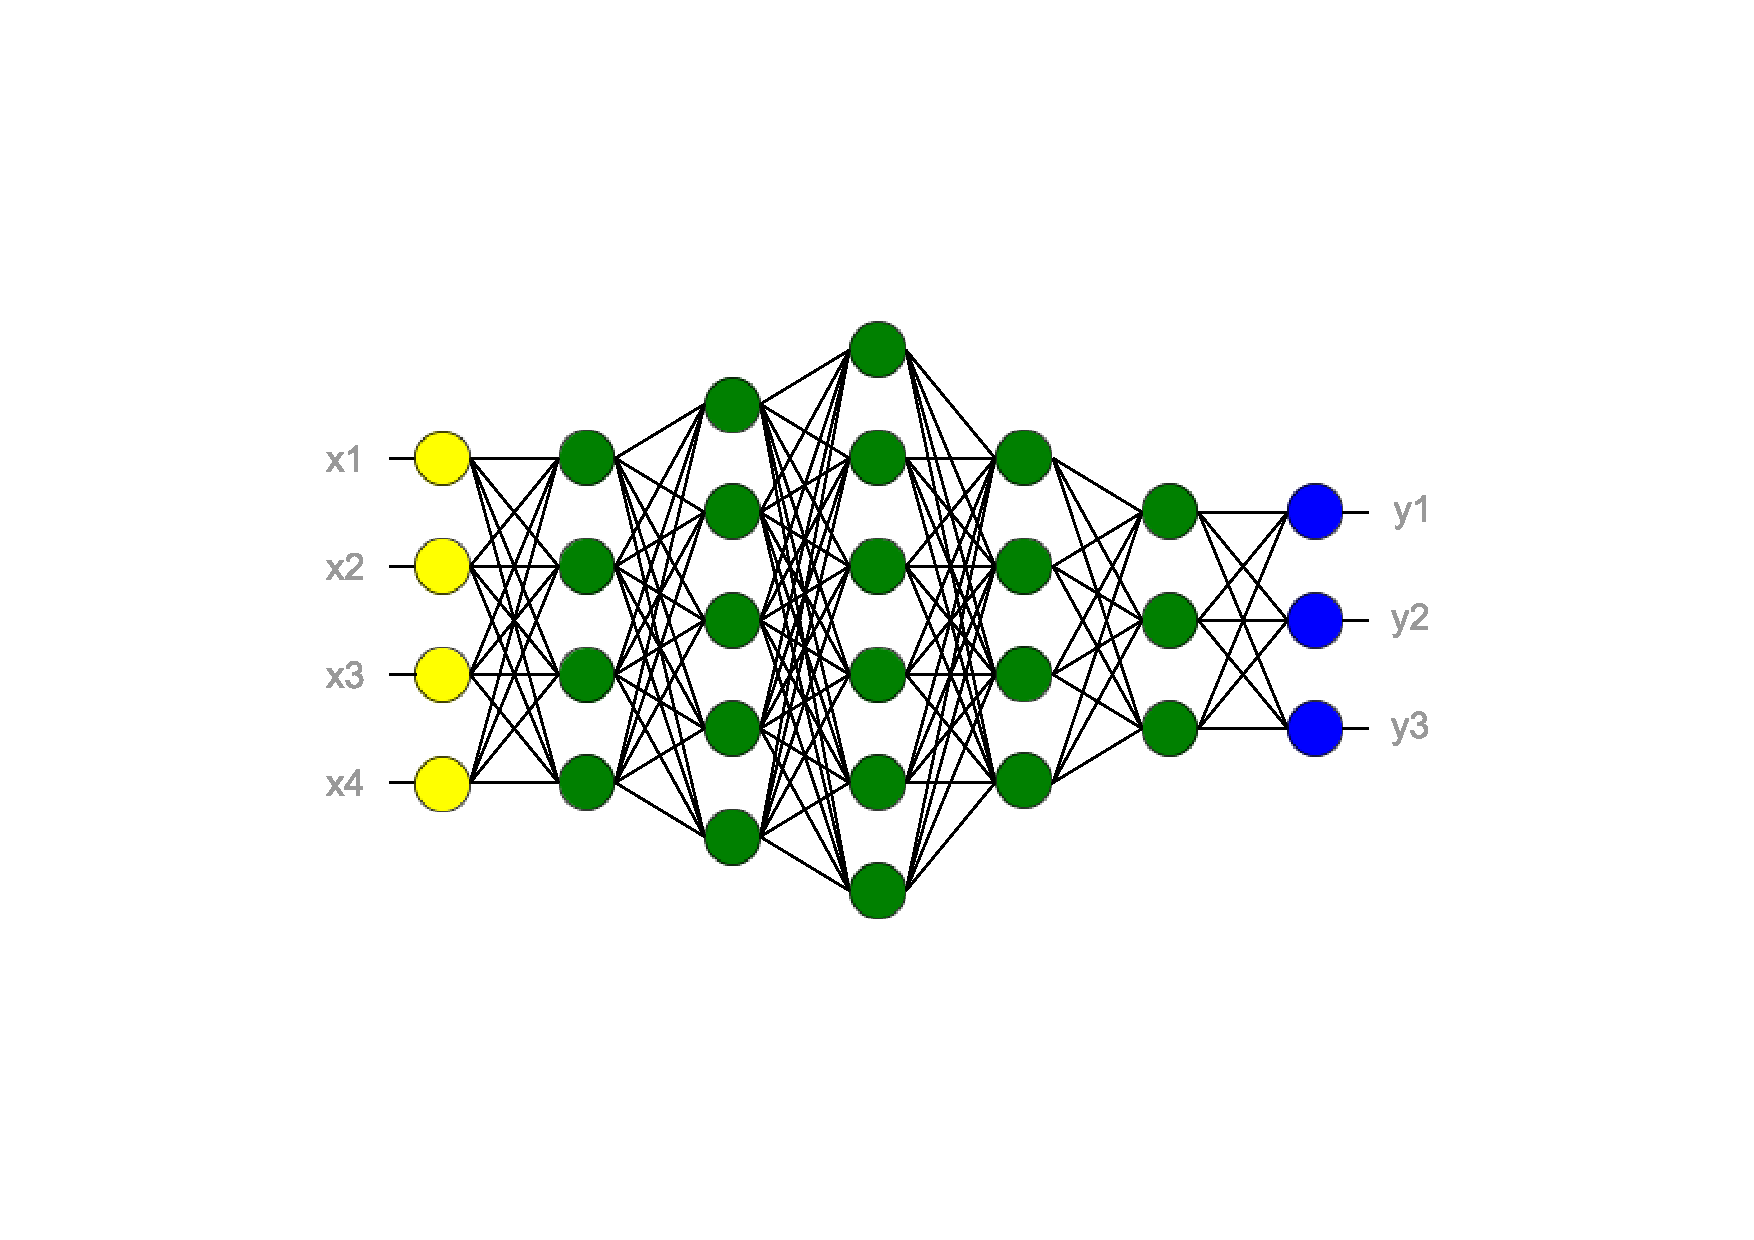
\includegraphics[width=0.8\textwidth]{mlp}
\label{fig:mlp}
\end{figure}

\subsection{Redes convolucionais}
Na década de 1970 as redes convolucionais já estavam sendo desenvolvidas. Uma aplicação famosa se deu em 1989, quando LeCun utilizou uma rede desse tipo em escala comercial para automatizar a leitura de talão de cheques. Apesar disso os algoritmos de treinamento ainda eram precários e a técnica acabou sendo abandonada em detrimento de técnicas superficiais, como \textit{Support Vector Machines}.

Com o aumento drástico do poder de processamento essas redes ultrapassaram seus predecessores e ganharam destaque novamente após o trabalho de Hinton \cite{hintonDL} em 2006, que estabeleceu uma base sólida para o treinamento de grandes redes convolucionais. Essa contribuição mudou o paradigma do aprendizado de máquina no que se refere à extração de características e se mostra ainda hoje como estado da arte. 

Nessas estruturas definem-se filtros, na forma de matrizes, que são convoluídas com uma imagem (proveniente da camada anterior) e resultam em outra imagem, com algum aspecto realçado. Em geral, muitos filtros são definidos e há, portanto, muitas imagens de saída para cada nível de convolução, o que aumenta drasticamente a dimensionalidade da rede. Nesses casos é comum utilizar um processo de \textit{max-pooling} em que seleciona-se diversos pixels (sob máscara quadrada) e retorna-se um único pixel cujo valor é o máximo dos pixels do conjunto original.

A grande vantagem dessas redes é reduzir o número de parâmetros geral do modelo e ainda assim manter uma alta capacidade de aprendizado. Elas também possibilitam que estruturas locais sejam encontradas mais facilmente de maneira a compor um descritor mais complexo e discriminativo para imagens.

Além disso, existe a vantagem da invariância à translação: em uma rede MLP, para encontrar faces em uma imagem, seria necessário amostras em todas as posições da imagem possíveis. Já em uma rede convolucional esse problema é resolvido através da convolução e amostragem e garante esse aspecto fundamental para detecção de objetos.

\begin{figure}[h]
\caption{Exemplo de rede convolucional duas camadas convolucionais e de max-pooling}
\centering
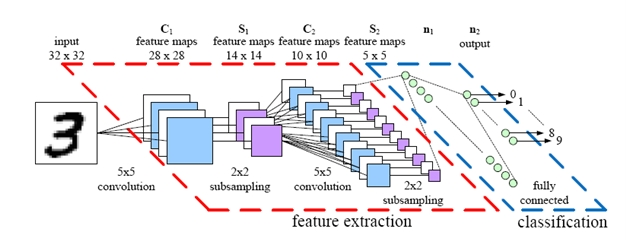
\includegraphics[width=0.8\textwidth]{convnet}
\label{fig:convnet}
\end{figure}

\section{Organização}
O trabalho é organizado em três soluções. A primeira é fundamentada nos métodos tradicionais de visão computacional e aprendizado de máquina. Divide-se o algoritmo em localização de candidatos à pessoas e posterior extração de características, desenvolvida manualmente, e classificação através de \textit{Support Vector Machines}.

Em seguida, propõe-se um método que emprega o mesmo algoritmo tradicional de localização de candidatos porém utiliza métodos de aprendizado profundo para o processo de classificação. Compreende-se que o classificador encontra de maneira automática um descritor de caracterísitcas específico para o conjunto de dados do problema nas camadas de convolução. A classificação própriamente dita se dá nas camadas finais da rede profunda.

A terceira solução é concebida utilizando-se integralmente soluções de aprendizado profundo: tanto localização como detecção. Uma rede de convolução é utilizada e recebe como entrada a imagem completa do ambiente industrial. A saída é uma máscara indicando a posição das pessoas encontradas na imagem. Essa rede é treinada utilizando um amplo conjunto de quadros e algortimo de propagação reversa de erros.

Tendo implementado os métodos e de posse de um dataset grande o suficiente para o treinamento das redes profundas, espera-se avaliar a performance de cada opção proposta e verificar qual a melhor solução, além de observar o impacto da utilização das redes profundas em diferentes etapas do sistema.




